% !Mode:: "TeX:UTF-8"
% !TEX root = ../Book.tex

\clearpage

%\setcounter{chapter}{4}\setcounter{page}{1}
\fancyhead[EC]{\small\small\thepage\rm\hfill \small 深度学习在多元时间序列上的应用 \hfill}
\fancyhead[OC]{\rm\hfill\small 第4章\quad 深度生成网络 \hfill\thepage}

\chapter{深度生成网络}
我们知道,机器学习领域中遇到的大部分模型可以分成两大类——判别模型(Discriminative Model)和生成模型(Generative Model)。
\begin{itemize}
	\setlength{\itemsep}{0pt}
    \setlength{\parsep}{0pt}
    \setlength{\parskip}{0pt}
	\item \textbf{判别模型}:判别模型本质上学习的是输入数据$\Vx$到输出数据$\Vy$的映射函数;而从概率论的角度来看学习的是条件概率分布$p(\Vy|\Vx)$。
	\item \textbf{生成模型}:生成模型的学习目标是输入数据和输出数据的联合概率分布$p(\Vx,y)$,根据条件概率分布我们不仅可以通过贝叶斯公式得到条件概率分布$p(y|\Vx)$,还可以对联合概率分布$p(\Vx,y)$进行采样从而得到新的样本数据;在没有标签的无监督学习场景下,生成模型学习的是输入数据的分布$p(\Vx)$。
\end{itemize}
与判别模型相比,生成模型的最大优点是它可以解释样本数据背后的的数据源,并产生新的样本数据。前面两个章节中介绍的CNN和RNN都属于判别模型,在本章我们将介绍一些属于生成模型的深度神经网络,它们在多元时间序列上也有着广泛的应用。


\section{生成模型}
在建立生成模型的时候,我们首先假设所有的样本数据来自于某个未知的分布$p_{r}$($r$代表real,对于有监督学习可以把标签看作样本数据的一部分);然后设计一个含有参数$\bm{\theta}$的分布$p_{\theta}$去近似$p_{r}$。模型训练的过程就是不断优化$\bm{\theta}$的过程。$p_{\theta}$的学习一般有两种方式:
\begin{itemize}
	\setlength{\itemsep}{0pt}
    \setlength{\parsep}{0pt}
    \setlength{\parskip}{0pt}
	\item 由最大似然估计直接学习$p_{\theta}$。
	\item 学习一个函数$g_{\theta}$,该函数把某个已知的分布$\mathcal{Z}$(例如正态分布、均匀分布等)变换成$p_{\theta}$,即$p_{\theta}=g_{\theta}(\mathcal{Z})\approx p_{r}$。
\end{itemize}

\subsubsection{通过最大似然估计直接学习样本数据真实分布}
在第一种方式中,最大似然估计的目标函数等价于最小化KL散度:
\begin{eqnarray}
\lim_{n\to\infty} \max_{\bm{\theta}}\frac{1}{n}\sum_{i=1}^{n}\log p_{\bm{\theta}}(\Vx^{(i)})
&=& \max_{\bm{\theta}}\int_{\Vx}p_{r}(\Vx)\log p_{\theta}(\Vx)dx\\
&=& \min_{\bm{\theta}}-\int_{\Vx}p_{r}(\Vx)\log p_{\theta}(\Vx)dx\\
&=& \min_{\bm{\theta}}\int_{\Vx}p_{r}(\Vx)\log p_{r}(\Vx)dx - \int_{\Vx}p_{r}(\Vx)\log p_{\theta}(\Vx)dx\\
&=& \min_{\bm{\theta}}\int_{\Vx}p_{r}(\Vx)\log \frac{p_{r}(\Vx)dx}{p_{\theta}(\Vx)dx}\\
&=& \min_{\bm{\theta}} D_{KL}(p_{r}(\Vx)\|p_{\theta}(\Vx))
\end{eqnarray}
其中$n$表示样本总数,$\Vx^{(i)}$表示样本数据中的第$i$个样本,$D_{KL}$表示KL散度。第一种方式十分直观,但有以下几个缺点:
\begin{enumerate}
	\setlength{\itemsep}{0pt}
    \setlength{\parsep}{0pt}
    \setlength{\parskip}{0pt}
	\item 以KL散度作为优化标准会要求样本在$p_{r}$和$p_{\theta}$上都有定义,否则KL散度将无法在这两个分布上定义。如果对于某个样本$\Vx$,$p_{\theta}(\Vx)=0$且$p_{r}(\Vx)>0$则$D_{KL}$会趋于$+\infty$。虽然我们可以通过对$p_{\theta}$添加随机噪声来避免这种情况的发生,但随机噪声一方面会降低模型的准确度,另一方面也会提高模型的训练复杂度。
	\item 训练中或训练后可能会遇到需要对$p_{\theta}$进行采样的情况,若$p_{\theta}$本身比较复杂将会导致采样变得困难,有时不得不使用马尔可夫链蒙特卡洛方法(Markov chain Monte Carlo, MCMC)。
\end{enumerate}
在深度学习相关的领域中,使用这种方式学习的生成模型常见的有玻尔兹曼机(Boltzmann Machine)、受限玻尔兹曼机(Restricted Boltzmann Machine, RBM)、深度信念网络(Deep Brief Network, DBN)、深度玻尔兹曼机(Deep Boltzmann Machine, DBM)等等。这些模型在多元时间序列处理中较少使用,本章将在最后部分对其进行简单介绍。

\subsubsection{通过变换函数间接学习样本数据真实分布}
针对第一种方式的不足之处,第二种通过变换函数间接学习样本数据真实分布的方法便被设计了出来。第二种方式中的变换函数$g_{\theta}$通常又被称为发生器(Generator)。由这种方式训练得到的模型最大的优点是样本的生成非常容易——只需要对已知的分布$\mathcal{Z}$采样得到样本$\Vz$,然后对$\Vz$进行变换得到的$g_{\theta}(\Vz)$便是来自于$p_{\theta}$的样本。这样的优点同时也会带来显而易见的缺点——我们并不能显式的得到$p_{\theta}$的表达式。在本书的第二部分“多元时间序列”中我们会看到,这一缺点在实践应用中并不会造成太多困难。

既然我们的计划是通过训练$g_{\theta}$来让$p_{\theta}$趋于$p_{r}$,那么我们就需要找到衡量两个分布相似度的标准。在第一种方式中,最大似然估计暗含的衡量是KL散度,虽然KL散度是最常用的,但事实上计算分布相似度的方法有很多:
\begin{itemize}
	\setlength{\itemsep}{0pt}
    \setlength{\parsep}{0pt}
    \setlength{\parskip}{0pt}
	\item Total Variation距离
	\begin{eqnarray}
	\delta(p_{r},p_{\theta}) = \sup_{\SetA\in\Sigma}(p_{r}(A) - p_{\theta}(\SetA))
	\end{eqnarray}
	其中$\Sigma$表示sigma-代数,是样本数据空间的子集$\SetA$的非空集合,这部分内容属于测度论,已经超出了本书的讨论范畴,在此就不展开介绍了。直观理解的话可以认为TV距离指的是两个概率分布对同一个事件分配概率的最大差值。\\
	\item Kullback-Leibler散度
	\begin{eqnarray}
	D_{KL}(p_{r}\|p_{\theta}) = \int_{\Vx}\log\Big{(} \frac{p_{r}(\Vx)}{p_{\theta}(\Vx)} \Big{)}p_{r}(\Vx)dx
	\end{eqnarray}
	KL散度是两个分布之间的相对熵,上式的意义是当使用$p_{\theta}$来近似$p_{r}$时产生的信息损耗。KL散度的主要问题是:1.非对称;2.之前我们已经提到过的,当两个分布相距较远没有重叠的时候KL散度趋于$+\infty$,或者说没有意义。\\
	\item Jenson-Shannon散度
	\begin{eqnarray}
	D_{JS}(p_{r},p_{\theta}) = \frac{1}{2}D_{KL}(p_{r}\|p_{m}) + \frac{1}{2}D_{KL}(p_{\theta}\|p_{m})
	\end{eqnarray}
	其中$p_{m}=\frac{1}{2}p_{r}+\frac{1}{2}p_{\theta}$。JS散度建立在KL散度之上,解决了KL散度作为差异度量却非对称的问题,同时当KL散度趋于$+\infty$时JS散度为一个常数。这在模型的学习训练过程中是非常严重的问题,因为此时该处的梯度为$0$,训练将无法继续。\\
	\item Wasserstein距离
	\begin{eqnarray}
	W(p_{r},p_{\theta}) = \inf_{\gamma\in\Pi(p_{r},p_{\theta})} \SetE_{(\Vx,\Vy)\sim\gamma}[\|\Vx-\Vy\|] \label{eqn:Wasserstein}
	\end{eqnarray}
	其中$\gamma(\Vx,\Vy)$表示边缘分布分别为$p_{r}$与$p_{\theta}$的联合分布,$\Pi(p_{r},p_{\theta})$表示$p_{r}$与$p_{\theta}$所有可能的联合分布,$\|\Vx-\Vy\|$表示$\Vx$与$\Vy$的欧氏距离。从定义式上Wasserstein距离很难理解,但事实上Wasserstein距离在现实中有很明确的物理意义。Wasserstein距离又被称为Earth Mover距离,我们把两个概率分布看作是单位质量的“尘土”在某个空间中两种不同的堆叠方式,Earth Mover距离指的是从其中一种堆叠方式变换到另一种堆叠方式的“花费”,而“花费”定义为被移动的尘土质量乘以其移动距离(对于离散分布可能用“搬砖”来比喻会更加形象)。
\end{itemize}
不同的分布相似度度量实际上对应了不同的生成模型。生成对抗网络(Generative Adversarial Network, GAN)的目标函数是最小化$p_{r}$与$p_{\theta}$的JS散度;Wasserstein生成对抗网络(Wasserstein Generative Adversarial Network, WGAN)则试图最小化Wasserstein距离;基于能量的生成对抗网络(Energy-based Generative Adversarial Network, EBGAN)在训练过程中不断地优化两个分布之间的TV距离。

以上我们所提及生成模型都是把已知分布变换近似为真实分布,此外还有一类模型采用的是反向思路——把真实分布变换近似为已知分布来达到学习目标。这类模型的代表是变分自编码器(Variational Autoencoder, VAE)。VAE在训练过程中尽量使真实分布变换后的分布$g'_{\theta}(p_{r})$与已知分布$\mathcal{Z}$的KL散度最小。

上述生成模型在多元时间序列处理中都有用武之地,我们将在本章余下的部分中分别对WGAN、GAN、以及VAE进行重点介绍。

\section{Wasserstein生成对抗网络}
我们首先从最小化Wasserstein距离开始。选择Wasserstein距离是因为相比于其他几个常用的分布相似度度量,Wasserstein距离在深度学习场景中具有以下几个优点[\cite{pmlr-v70-arjovsky17a}]:
\begin{enumerate}
	\setlength{\itemsep}{0pt}
    \setlength{\parsep}{0pt}
    \setlength{\parskip}{0pt}
	\item 当$g_{\theta}$关于$\theta$连续时,Wasserstein距离$W(p_{r},p_{\theta})$也连续。
	\item 当$g_{\theta}$满足一定的假设时,$W(p_{r},p_{\theta})$处处连续且几乎处处可导。
	\item 如果一系列分布在TV距离、KL散度、JS散度下收敛,则其在Wasserstein距离的度量下也会收敛。
\end{enumerate}
优点1和2——连续且可导——在我们使用Wasserstein距离作为损失函数(Loss Function)时非常重要;优点3表明Wasserstein距离对于两个分布之间的变化更敏感。关于Wasserstein距离这几个性质的证明可以参见[\cite{pmlr-v70-arjovsky17a}]。

\subsection{Kantorovich-Rubinstein对偶}
接下来的问题就是我们如何求解Wasserstein距离。从Wasserstein距离的定义式(\ref{eqn:Wasserstein})可以看出其本身是一个有约束条件的最优化问题:
\begin{eqnarray}
W(p_{r},p_{\theta}) 
&=& \inf_{\gamma\in\Pi(p_{r},p_{\theta})} \SetE_{(\Vx,\Vy)\sim\gamma}[\|\Vx-\Vy\|]\\
\end{eqnarray}
其中约束条件$\gamma\in\Pi(p_{r},p_{\theta})$是比较难处理的部分,因为我们很难在分布空间中去寻找最优解。机器学习领域中常见的最优化问题一般都在向量空间(目标函数的梯度下降)或函数空间(GBM, XGBoost等)中,因此我们要把Wasserstein距离的求解转换到函数空间中。通过添加实值函数$f:\SetR^{n}\to\SetR$:
\begin{eqnarray}
W(p_{r},p_{\theta}) 
&=& \inf_{\gamma\in\Pi} \SetE_{(\Vx,\Vy)\sim\gamma}[\|\Vx-\Vy\|]\\
&=& \inf_{\gamma\in\Pi} \SetE_{(\Vx,\Vy)\sim\gamma}\big{[}\|\Vx-\Vy\| \nonumber\\ 
&& + \underbrace{\sup_{f}\SetE_{\Vs\sim p_{r}}[f(\Vs)] - \SetE_{\Vt\sim p_{\theta}}[f(\Vt)] - (f(\Vx)-f(\Vy))\big{]}}_{=
\begin{cases}
0 &\rm{if} \quad \gamma\in\pi \\
+\infty &\rm{otherwise}
\end{cases}
}\\
&=& \inf_{\gamma\in\Pi} \sup_{f} \SetE_{(\Vx,\Vy)\sim\gamma}\big{[}\|\Vx-\Vy\| \nonumber\\ 
&& + \SetE_{\Vs\sim p_{r}}[f(\Vs)] - \SetE_{\Vt\sim p_{\theta}}[f(\Vt)] - (f(\Vx)-f(\Vy))\big{]} \label{eqn:Wasserstein_Minimax}
\end{eqnarray}
观察最后得到的式(\ref{eqn:Wasserstein_Minimax}),我们会发现它跟支持向量机中的Minimax问题是一样的。对于Minimax问题始终有:
\begin{eqnarray}
\max\min\ (\sup_{f}\inf_{\gamma}) \leq \min\max\ (\inf_{\gamma}\sup_{f}) \label{eqn:Minimax}
\end{eqnarray}
这种“双层嵌套”的最优化问题可以通过计算机编程中的双重循环来理解:$\inf_{\gamma}\sup_{f}$的含义是对于每一个$\gamma$取值$\gamma_{i}$,分别通过选取$f$得到固定$\gamma_{i}$时表达式的最大值,然后从不同的$\gamma_{i}$所对应的最大值中选择最小的那个作为问题的解;而$\sup_{f}\inf_{\gamma}$则是先固定外层中不同的$f_{i}$,然后通过选取$\gamma$得到此时对应的表达式最小值,最后从这些最小值中选取最大的那个。式(\ref{eqn:Minimax})是显然成立的,因为
\begin{eqnarray}
&\min_{\Vy} f(\tilde{\Vx},\Vy) \leq f(\tilde{\Vx},\tilde{\Vy}) \leq \max_{\Vx} f(\Vx,\tilde{\Vy}) \quad \forall \tilde{\Vx},\tilde{\Vy} \\
&\max_{\Vx}\min_{\Vy} f(\Vx,\Vy) \leq \min_{\Vy}\max_{\Vx} f(\Vx,\Vy)
\end{eqnarray}
我们希望能够像求解支持向量机中的拉格朗日对偶问题那样交换$\inf_{\gamma}$和$\sup_{f}$。根据对拉格朗日对偶的理解我们知道,当目标函数满足一定的凹凸性条件时,交换$\inf$和$\sup$前后是相等的。式(\ref{eqn:Wasserstein_Minimax})便满足这样的条件[\cite{Villani07p}]。于是交换式(\ref{eqn:Wasserstein_Minimax})的$\inf_{\gamma}$和$\sup_{f}$可得
\begin{eqnarray}
W(p_{r},p_{\theta})
&=&  \sup_{f} \inf_{\gamma\in\Pi}\SetE_{(\Vx,\Vy)\sim\gamma}\big{[}\|\Vx-\Vy\| \nonumber\\ 
&& + \SetE_{\Vs\sim p_{r}}[f(\Vs)] - \SetE_{\Vt\sim p_{\theta}}[f(\Vt)] - (f(\Vx)-f(\Vy))\big{]}\\
&=& \sup_{f} \SetE_{\Vs\sim p_{r}}[f(\Vs)] - \SetE_{\Vt\sim p_{\theta}}[f(\Vt)] \nonumber\\
&& + \inf_{\gamma\in\Pi} \SetE_{(\Vx,\Vy)\sim\gamma}[\|\Vx-\Vy\| - (f(\Vx)-f(\Vy))] \label{eqn:Wasserstein_Maximin}
\end{eqnarray}
注意上式中的$\inf_{\gamma\in\Pi} \SetE_{(\Vx,\Vy)\sim\gamma}[\|\Vx-\Vy\| - (f(\Vx)-f(\Vy))]$项,有
\begin{eqnarray}
\inf_{\gamma\in\Pi} \SetE_{(\Vx,\Vy)\sim\gamma}[\|\Vx-\Vy\| - (f(\Vx)-f(\Vy))]
&=&
\begin{cases}
0, \quad &f(\Vx)-f(\Vy)\leq\|\Vx-\Vy\|\\
-\infty, \quad &f(\Vx)-f(\Vy)>\|\Vx-\Vy\|\\
\end{cases}
\end{eqnarray}
上式中的条件$f(\Vx)-f(\Vy)\leq\|\Vx-\Vy\|$事实上是对函数$f$的约束,它意味着$f$是1-Lipschitz连续的,即$\|f\|_{L}\leq1$。因此我们可以把式(\ref{eqn:Wasserstein_Maximin})中的$\inf_{\gamma\in\Pi} \SetE_{(\Vx,\Vy)\sim\gamma}[\|\Vx-\Vy\| - (f(\Vx)-f(\Vy))]$项替换成对函数$f$的约束条件$\|f\|_{L}\leq1$得到
\begin{eqnarray}
W(p_{r},p_{\theta}) = \sup_{\|f\|_{L}\leq1} \SetE_{\Vs\sim p_{r}}[f(\Vs)] - \SetE_{\Vt\sim p_{\theta}}[f(\Vt)] \label{eqn:Kantorovich-Rubinstein_duality}
\end{eqnarray}
式(\ref{eqn:Kantorovich-Rubinstein_duality})被称为Kantorovich-Rubinstein对偶[\cite{Villani07p}]。

\subsection{WGAN}
接下来我们在Kantorovich-Rubinstein对偶的基础上给出Wasserstein的具体求解算法。Kantorovich-Rubinstein对偶式(\ref{eqn:Kantorovich-Rubinstein_duality})之所以难以求解是因为其中存在的约束条件$\|f\|_{L}\leq1$。该约束条件意味着需要在整个1-Lipschitz连续函数集合上寻找最优解。这显然是不可能的。我们只能在1-Lipschitz连续函数集合的某个子集$\{f_{\Vw}\}_{\Vw\in\MW}\subset\{f\}_{\|f\|_{L}\leq1}$中搜寻(其中$\Vw$表示$f$的参数)。即使如此,找到$\{f_{\Vw}\}_{\Vw\in\MW}\subset\{f\}_{\|f\|_{L}\leq1}$这样一个集合也是困难重重,因此不得不把从$\|f\|_{L}\leq1$放宽为$\|f\|_{L}\leq K$,其中$K$为某个未知的正整数。在接下来的分析中会看到$K$的具体取值并不会影响我们最关心的$p_{\theta}$求解,$K$只要存在即可。于是对于这样一个可以“随意取值”的$K$,找到一个$K$-Lipschitz连续函数集合的子集$\{f_{\Vw}\}_{\Vw\in\MW}\subset\{f\}_{\|f\|_{L}\leq K}$就容易多了。

由Lipschitz连续性的定义可知,$K$-Lipschitz连续的函数$f:\SetX\to\SetY$满足
\begin{eqnarray}
d_{\SetY}(f(\Vx_{1}),\Vx_{2}) \leq Kd_{\SetX}(\Vx_{1},\Vx_{2})
\end{eqnarray}
其中$d_{\SetX}$和$d_{\SetY}$分别表示在$\SetX$和$\SetY$空间的距离。如果把式(\ref{eqn:Kantorovich-Rubinstein_duality})中对$f$的约束条件从1-Lipschitz连续放宽为$K$-Lipschitz连续,则Wasserstein距离也会相应地扩大$K$倍:
\begin{eqnarray}
K\cdot W(p_{r},p_{\theta}) = \sup_{\|f\|_{L}\leq K} \SetE_{\Vx\sim p_{r}}[f(\Vx)] - \SetE_{\Vx\sim p_{\theta}}[f(\Vx)]
\end{eqnarray}
上式中由于约束条件$\|f\|_{L}\leq K$的存在而无法计算,于是我们使用一组带参数$\Vw$的函数$\{f_{\Vw}\}_{\Vw\in\MW}$近似$K$-Lipschitz连续的函数,从而消除约束条件$\|f\|_{L}\leq K$:
\begin{eqnarray}
\max_{\Vw\in\MW}\SetE_{\Vx\sim p_{r}}[f_{\Vw}(\Vx)] - \SetE_{\Vx\sim p_{\theta}}[f_{\Vw}(\Vx)] 
&\leq& \sup_{\|f\|_{L}\leq K} \SetE_{\Vx\sim p_{r}}[f(\Vx)] - \SetE_{\Vx\sim p_{\theta}}[f(\Vx)] \label{eqn:KR_Duality_K-Lipschitz}\\
&=& K\cdot W(p_{r},p_{\theta})\label{eqn:K_times_gradient}
\end{eqnarray}
如果$\{f_{\Vw}\}_{\Vw\in\MW}$对$K$-Lipschitz连续函数近似的足够好,式(\ref{eqn:KR_Duality_K-Lipschitz})就越接近于取等号。此时问题已经转换为式(\ref{eqn:KR_Duality_K-Lipschitz})不等号的左边部分
\begin{eqnarray}
\max_{\Vw\in\MW}\SetE_{\Vx\sim p_{r}}[f_{\Vw}(\Vx)] - \SetE_{\Vx\sim p_{\theta}}[f_{\Vw}(\Vx)]\label{eqn:WGAN_problem}
\end{eqnarray}
对于该最优化问题,我们只需在参数$\Vw$空间上进行梯度下降。

现在我们来解决$K$的“任意取值”问题。从式(\ref{eqn:K_times_gradient})可以看出,当我们在参数$\Vw$空间上进行梯度下降时,约束条件$\|f\|_{L}\leq K$下的梯度相当于$\|f\|_{L}\leq1$下的梯度放大$K$倍。而在梯度下降算法中,该梯度又会被梯度下降的步长(或者称为学习率,Learning Rate)放缩。因此无论$K$的真实取值是多少,只要保证在整个梯度下降的过程中$K$存在且不变,其所造成的影响都可以通过调整梯度下降的步长来消除,从而把约束条件$\|f\|_{L}\leq K$收缩回了$\|f\|_{L}\leq1$。最后的问题是如何保证$K$存在且不变?只要限制$\Vw$的取值范围始终在某一个区间即可。

现在让我们回到最初的问题——生成模型。我们希望通过训练变换函数$g_{\theta}$来让$p_{\theta}=g_{\theta}(\mathcal{Z})$趋于$p_{r}$,其中$\mathcal{Z}$为某个已知的简单分布。于是式(\ref{eqn:WGAN_problem})所描述的最优化问题就有两组参数$\Vw$和$\theta$需要优化,而两组参数的优化可以迭代交替进行:
\begin{itemize}
	\setlength{\itemsep}{0pt}
    \setlength{\parsep}{0pt}
    \setlength{\parskip}{0pt}
    \item 固定$\theta$,找到最优的$f_{\Vw}$使得$W(p_{r},p_{\theta})$最小。
    \item 固定$\Vw$,对$\theta$进行一次梯度下降。
\end{itemize}
重复上面两个步骤直到收敛。

鉴于神经网络强大的表达能力,我们使用两张网络分别近似$g_{\theta}$和$f_{\Vw}$。其中近似$g_{\theta}$的网络称为Generator,而近似$f_{\Vw}$的网络称为Critic。于是就得到了Wasserstein生成对抗网络。其算法框架如下:
\begin{center}
\begin{tabularx}{\textwidth}{X}
\toprule 
\textbf{{WGAN}算法框架}\\
\midrule
\textbf{输入}:已知分布$\mathcal{Z}$,梯度下降步长$\alpha$,$\Vw$梯度下降限制范围$c$,求$f_{\Vw}$最优解的迭代次数$n_{\rm{critic}}$\\
\textbf{初始}:$\Vw$和$\theta$的初始值\\
\textbf{重复}:当$\theta$未收敛时\\
\parbox{1\textwidth}{\begin{enumerate}[topsep=0pt]
    \setlength{\itemsep}{0pt}
    \setlength{\parsep}{0pt}
    \setlength{\parskip}{0pt}
    \item 计算$f_{\Vw}$的最优解,对$\Vw$进行$n_{\rm{critic}}$次梯度下降:
    \item $\quad$从训练集中随机采集$m$个样本$\{\Vx^{(i)}\}_{i=1}^{m}$
    \item $\quad$从已知分布$\mathcal{Z}$中随机采集$m$个样本$\{\Vz^{(i)}\}_{i=1}^{m}$
    \item $\quad$计算关于$\Vw$的梯度$G_{\Vw}\gets\nabla_{\Vw}\big{[} \frac{1}{m}\sum_{i=1}^{m}f_{\Vw}(\Vx^{(i)})-\frac{1}{m}\sum_{i=1}^{m}f_{\Vw}(g_{\theta}(\Vz^{(i)})) \big{]}$
    \item $\quad$更新参数$\Vw=\Vw + \alpha G_{\Vw}$
    \item $\quad$对参数$\Vw$进行梯度剪裁$\Vw\gets\rm{clip}(-c,c)$
    \item 优化$\theta$,对$g_{\theta}$进行一次梯度下降:
    \item $\quad$从已知分布$\mathcal{Z}$中随机采集$m$个样本$\{\Vz^{(i)}\}_{i=1}^{m}$
    \item $\quad$计算关于$\theta$的梯度$G_{\theta}\gets-\nabla_{\theta}\frac{1}{m}\sum_{i=1}^{m}f_{\Vw}(g_{\theta}(\Vz^{(i)}))$
    \item $\quad$更新参数$\theta=\theta + \alpha G_{\theta}$
\end{enumerate}}\\\bottomrule
\end{tabularx}
\end{center}

WGAN中的$g_{\theta}$网络是我们训练的目标,$f_{\Vw}$网络则扮演着辅助训练的角色。每当更新$\theta$得到新的$g_{\theta}$时,$f_{\Vw}$便估计此时的$g_{\theta}(\mathcal{Z})$与$p_{r}$的Wasserstein距离,如果二者的Wasserstein距离还不足够小,那就根据当前的Wasserstein距离计算$g_{\theta}$关于$\theta$的梯度,并更再次更新$\theta$。可以看出,$f_{\Vw}$网络在训练$g_{\theta}$网络的过程中扮演着“评论者”的角色——每当一个新的$g_{\theta}$提出来,$f_{\Vw}$便对其与$p_{r}$的Wasserstein距离进行一番“评论”,之后$g_{\theta}$会根据评论进行修改并提出新的$g_{\theta}$。这就是$f_{\Vw}$网络被称为Critic的原因。

从WGAN的架构上看,$g_{\theta}$和$f_{\Vw}$两张网络呈现出“对抗”的趋势。$g_{\theta}$不断地提出方案,$f_{\Vw}$不断地对其进行评价,直到二者达成一致(收敛)。像这样通过两张网络相互对抗来训练生成模型的架构是一类生成模型框架——生成对抗网络框架(图\ref{fig:GAN_framework})。这一类模型都源自于生成对抗网络(GAN),在GAN中两张网络的对抗意味更加明显。
\begin{figure}[ht]
\centering
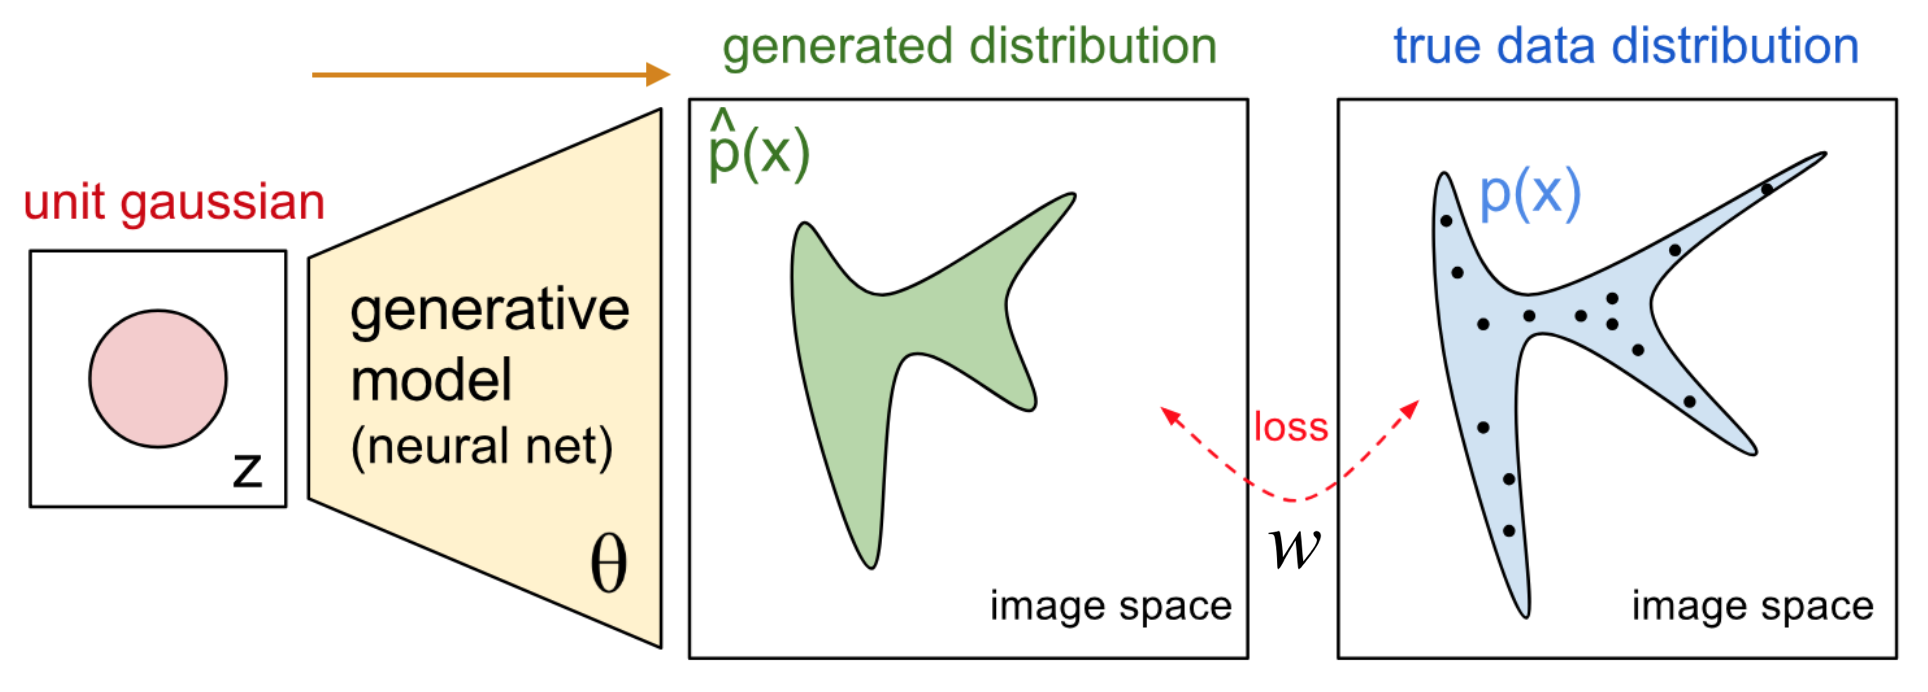
\includegraphics[scale=0.4]{{figures/gen_models_GAN.png}}
\caption{生成对抗网络框架}
\label{fig:GAN_framework}
\end{figure}

\section{生成对抗网络}
与WGAN一样,GAN也是由两张网络构成——$g_{\theta}$和$f_{\Vw}$。GAN中$g_{\theta}$网络的作用依然是把已知分布$\mathcal{Z}$变换为目标分布$p_{r}$,而$f_{\Vw}$网络则与WGAN完全不同。GAN中的$f_{\Vw}$扮演的是“判定者”的角色,它像一个裁判那样判定$g_{\theta}$输出的样本是否来自于训练集背后的真实分布$p_{r}$。因此$f_{\Vw}$接受$g_{\theta}$的输出,并输出一个表示其属于目标分布$p_{r}$的概率。我们把GAN中的$g_{\theta}$网络依然称为Generator,而$f_{\Vw}$网络则称为Discriminator。两张神经网络的优化目标分别为:
\begin{itemize}
	\setlength{\itemsep}{0pt}
    \setlength{\parsep}{0pt}
    \setlength{\parskip}{0pt}
	\item Discriminator的优化目标是
		\begin{eqnarray}
		\max_{\Vw} \SetE_{\Vx\sim p_{r}}\big{[}\log f_{\Vw}(\Vx)\big{]} + \SetE_{\Vz\sim\mathcal{Z}}\big{[}\log(1-f_{\Vw}(g_{\theta}(\Vz)))\big{]}
		\end{eqnarray}
	\item Generator的优化目标是
		\begin{eqnarray}
		\min_{\theta} \SetE_{\Vz\sim\mathcal{Z}}\big{[}\log(1-f_{\Vw}(g_{\theta}(\Vz)))\big{]}
		\end{eqnarray}
\end{itemize}
注意GAN中的$f_{\Vw}$作为Discriminator其输出是$0$到$1$之间的概率值。

GAN的训练过程与WGAN十分类似:
\begin{itemize}
	\setlength{\itemsep}{0pt}
    \setlength{\parsep}{0pt}
    \setlength{\parskip}{0pt}
    \item 固定$\theta$,找到最优的$f_{\Vw}$使得Discriminator的判别准确率最高。
    \item 固定$\Vw$,将$\SetE_{\Vz\sim\mathcal{Z}}\big{[}\log(1-f_{\Vw}(g_{\theta}(\Vz)))\big{]}$作为$g_{\theta}$的loss对$\theta$进行一次梯度下降。
\end{itemize}
重复上面两个步骤直到收敛。GAN的算法框架如下:
\begin{center}
\begin{tabularx}{\textwidth}{X}
\toprule 
\textbf{{GAN}算法框架}\\
\midrule
\textbf{输入}:已知分布$\mathcal{Z}$,梯度下降步长$\alpha$,求$f_{\Vw}$最优解的迭代次数$n_{\rm{discriminator}}$\\
\textbf{初始}:$\Vw$和$\theta$的初始值\\
\textbf{重复}:当$\theta$未收敛时\\
\parbox{1\textwidth}{\begin{enumerate}[topsep=0pt]
    \setlength{\itemsep}{0pt}
    \setlength{\parsep}{0pt}
    \setlength{\parskip}{0pt}
    \item 训练$f_{\Vw}$,在$\Vw$上进行$n_{\rm{discriminator}}$次梯度下降:
    \item $\quad$从训练集中随机采集$m$个样本$\{\Vx^{(i)}\}_{i=1}^{m}$
    \item $\quad$从已知分布$\mathcal{Z}$中随机采集$m$个样本$\{\Vz^{(i)}\}_{i=1}^{m}$
    \item $\quad$计算关于$\Vw$的梯度$G_{\Vw}\gets\nabla_{\Vw}\frac{1}{m}\sum_{i=1}^{m}\big{[} \log f_{\Vw}(\Vx^{(i)})+\log(1-f_{\Vw}(g_{\theta}(\Vz^{(i)}))) \big{]}$
    \item $\quad$更新参数$\Vw=\Vw + \alpha G_{\Vw}$
    \item 训练$g_{\theta}$,在$\theta$上进行一次梯度下降:
    \item $\quad$从已知分布$\mathcal{Z}$中随机采集$m$个样本$\{\Vz^{(i)}\}_{i=1}^{m}$
    \item $\quad$计算关于$\theta$的梯度$G_{\theta}\gets\nabla_{\theta}\frac{1}{m}\sum_{i=1}^{m}\log(1-f_{\Vw}(g_{\theta}(\Vz^{(i)})))$
    \item $\quad$更新参数$\theta=\theta + \alpha G_{\theta}$
\end{enumerate}}\\\bottomrule
\end{tabularx}
\end{center}

在具体的代码实现中,对于同一个$p_{r}$,GAN和WGAN唯一显著的不同是GAN在WGAN的$f_{\Vw}$网络后面添加了一个Logistic层,从而把$f_{\Vw}$的输出限定在了$(0,1)$区间。这一点点不同使得整个模型的意义发生了巨大变化。在本章第一节我们曾经提到过GAN的目标函数是最小化$g_{\theta}(\mathcal{Z})$与$p_{r}$的JS散度。事实上GAN在其训练过程中并没显式地沿着减小JS散度的方向去优化,GAN只是在$\theta$最终收敛时$g_{\theta}(\mathcal{Z})$与$p_{r}$的JS散度达到最小[\cite{goodfellow_14}]。


\section{变分自编码器}
前面两节中我们介绍的WGAN和GAN都是把某个已知分布变换近似为真实分布来得到生成模型(图\ref{fig:GAN_framework})。此外还有一类模型采用的是反向思路——把真实分布变换近似为已知分布来达到学习目标(图\ref{fig:VAE_framework},注意图中左上角的箭头方向)。这类模型的代表是变分自编码器(VAE)。VAE在训练过程中尽量使真实分布变换后的分布与已知分布的KL散度最小。
\begin{figure}[ht]
\centering
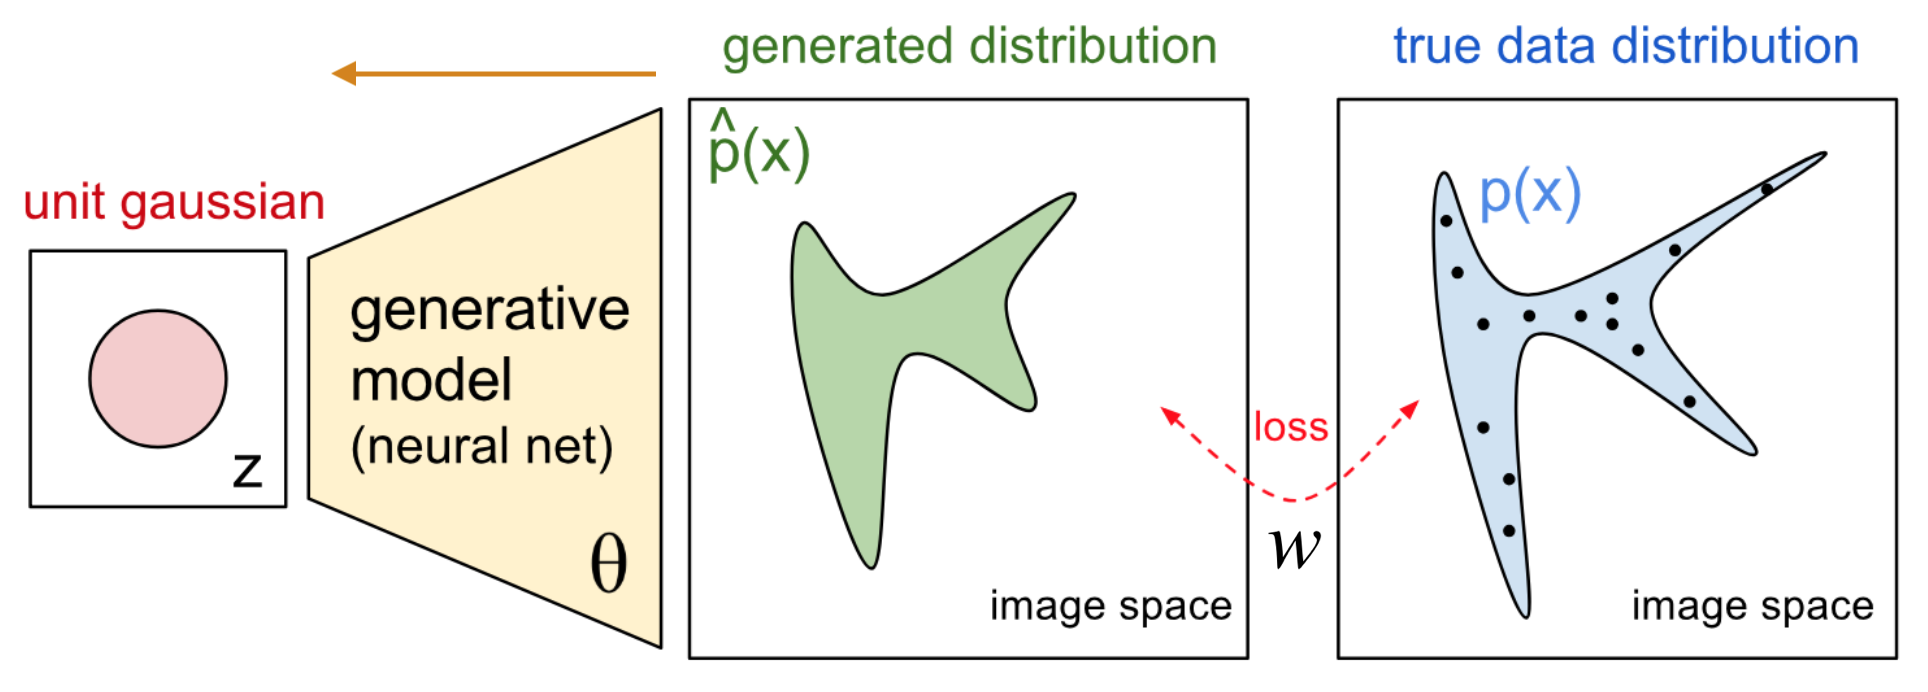
\includegraphics[scale=0.4]{{figures/gen_models_VAE.png}}
\caption{变分自编码器框架}
\label{fig:VAE_framework}
\end{figure}

\subsection{VAE架构}
VAE同样由两张神经网络构成:第一张网络$q_{\theta}(\Vz|\Vx)$称为编码器(Encoder),它把来自于目标分布$p_{r}$(训练集)的样本$\Vx$编码为来自已知分布$\mathcal{Z}$的样本$\Vz$;第二张网络$p_{\Vw}(\Vx|\Vz)$称为解码器(Decoder),它把Encoder编码得到的$\Vz$还原为$\Vx$。解码器的存在有两个意义:
\begin{itemize}
	\setlength{\itemsep}{0pt}
    \setlength{\parsep}{0pt}
    \setlength{\parskip}{0pt}
	\item 辅助编码器对目标分布$p_{r}$向已知分布$\mathcal{Z}$的变换\\
			编码器在变换分布的过程中难免丢失信息,如果信息丢失过多则解码器将很难还原。解码器会根据对原始输入的还原情况评估信息的丢失程度并传递给编码器,从而辅助其改进。
	\item 训练完成后解码器即为目标生成模型(即GAN框架中的Generator)\\
			训练完成之后若需要生成来自于$p_{r}$的样本,只需对已知分布$\mathcal{Z}$采样并输入到解码器中,对应的解码器输出即为来自于$p_{r}$的样本。
\end{itemize}
至此VAE和自编码器(Autoencoder, AE)并无区别,这是因为有一个问题还未解决——编码器如何将目标分布$p_{r}$变换为已知分布$\mathcal{Z}$呢?自编码器的学习目标是最大化解码器的还原程度:
\begin{eqnarray}
\max_{\theta,\Vw}\SetE_{\Vz\sim q_{\theta}(\Vz|\Vx)}\big{[} \log p_{\Vw}(\Vx|\Vz) \big{]}
\end{eqnarray}
既然我们希望的是编码器$q_{\theta}(\Vz|\Vx)$的输出$\Vz$来自于已知分布$\mathcal{Z}$,那么只要$q_{\theta}(\Vz|\Vx)\approx\mathcal{Z}$便可以满足我们的要求,因此我们可以把此作为学习目标的一部分。选择KL散度作为分布相似度的衡量,则VAE的学习目标为
\begin{eqnarray}
\max_{\theta,\Vw}\SetE_{\Vz\sim q_{\theta}(\Vz|\Vx)}\big{[} \log p_{\Vw}(\Vx|\Vz) \big{]} - D_{KL}(q_{\theta}(\Vz|\Vx)\|\mathcal{Z}) \label{eqn:VAE_loss}
\end{eqnarray}
上式(\ref{eqn:VAE_loss})的含义是:解码器对编码器变换之后样本的还原要尽可能的高,且编码器变换之后的样本要尽可能的服从已知分布$\mathcal{Z}$。

可以看出,编码器和解码器两张网络在VAE的架构中相比于对抗,更多的是协作。

我想如果读者是第一次接触VAE,那么你肯定会问:变分自编码器中的“变分”体现在哪里?变分的思想是从概率模型(Probablity Model)的角度体现出来的。这是对VAE的另一种解读。

\subsection{变分与概率图模型}
从概率图模型的角度我们便可以看到VAE中所蕴含的变分思想。概率图模型(图\ref{fig:VAE_graphical_model})认为数据$\Vx$的分布收到其背后的隐变量$\Vz$的影响,即$p(\Vx|\Vz)$,而二者的联合分布为$p(\Vx,\Vz)=p(\Vx|\Vx)p(\Vz)$。
\begin{figure}[ht]
\centering
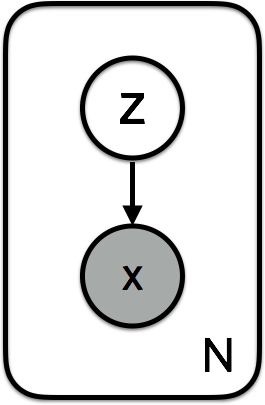
\includegraphics[scale=0.4]{{figures/VAE_graphical_model.png}}
\caption{变分自编码器的概率图模型}
\label{fig:VAE_graphical_model}
\end{figure}
于是$\Vx$的样本生成过程分为两步:
\begin{enumerate}
	\setlength{\itemsep}{0pt}
    \setlength{\parsep}{0pt}
    \setlength{\parskip}{0pt}
	\item 对隐变量采样得到$\Vz_{i}\sim p(\Vz)$
	\item 对数据采样得到$\Vx_{i}\sim p(\Vx|\Vz_{i})$
\end{enumerate}
现在我们要做的事情是对这个概率图模型进行推断,希望根据观测到的样本数据$\Vx$来还原出背后的隐变量分布,即$\Vz$的后验概率$p(\Vz|\Vx)$。根据贝叶斯公式我们有
\begin{eqnarray}
p(\Vz|\Vx) = \frac{p(\Vx|\Vz)p(\Vz)}{p(\Vx)}
\end{eqnarray}
对于上式右边部分的分母$p(\Vx)$有$p(\Vx)=\int_{\Vz}p(\Vx|\Vz)p(\Vz)d\Vz$,代入上式可得
\begin{eqnarray}
p(\Vz|\Vx) = \frac{p(\Vx|\Vz)p(\Vz)}{\int_{\Vz}p(\Vx|\Vz)p(\Vz)d\Vz}
\end{eqnarray}
然而求解$\int_{\Vz}p(\Vx|\Vz)p(\Vz)d\Vz$需要遍历整个$\mathcal{Z}$空间,这在求解实际问题中是不可能的,因此我们需要对后验概率$p(\Vz|\Vx)$进行近似求解。对于这类问题一般有两个方法——马尔可夫链蒙特卡洛法和变分推断法。马尔可夫链蒙特卡洛法精度较高,但由于要生成大量的采样其时间消耗巨大;而变分推断法相对精度不高但求解速度很快。在这里我们选择后者。

变分推断通过一个分布族$q_{\lambda}(\Vz|\Vx)$来近似后验概率$p(\Vz|\Vx)$,其中$\lambda$表征了分布族中的不同分布。最常用的分布族之一就是高斯分布族,此时$\lambda=(\mu,\sigma^{2})$。既然我们要在分布族$q_{\lambda}(\Vz|\Vx)$中找到最接近$p(\Vz|\Vx)$的分布$q_{\lambda}^{*}(\Vz|\Vx)$,这就又遇到了衡量分布相似度的问题,在变分推断中我们选择的是最常见的KL散度。于是原问题现在转化为了一个最优化问题:
\begin{eqnarray}
q_{\lambda}^{*}(\Vz|\Vx) = \mathop{\argmin}_{\lambda}D_{KL}(q_{\lambda}(\Vz|\Vx)\|p(\Vz|\Vx))
\end{eqnarray}
根据KL散度的定义有
\begin{eqnarray}
D_{KL}(q_{\lambda}(\Vz|\Vx)\|p(\Vz|\Vx))
&=& \int_{\Vz}\log\Big{(} \frac{q_{\lambda}(\Vz|\Vx)}{p(\Vz|\Vx)} \Big{)}q_{\lambda}(\Vz|\Vx)d\Vz \nonumber\\
&=& \int_{\Vz}\log\Big{(} \frac{q_{\lambda}(\Vz|\Vx)}{p(\Vx,\Vz)}p(\Vx) \Big{)}q_{\lambda}(\Vz|\Vx)d\Vz \nonumber\\
&=& \int_{\Vz}\log\Big{(} q_{\lambda}(\Vz|\Vx) - p(\Vx,\Vz) + p(\Vx) \Big{)}q_{\lambda}(\Vz|\Vx)d\Vz \nonumber\\
&=& \SetE_{\Vz\sim q}[\log q_{\lambda}(\Vz|\Vx)] - \SetE_{\Vz\sim q}[\log p(\Vx,\Vz)] + \int_{\Vz}\log p(\Vx)q_{\lambda}(\Vz|\Vx)d\Vz \nonumber\\
&=& \SetE_{\Vz\sim q}[\log q_{\lambda}(\Vz|\Vx)] - \SetE_{\Vz\sim q}[\log p(\Vx,\Vz)] + \log p(\Vx) \label{eqn:ELBO_1}
\end{eqnarray}
上式(\ref{eqn:ELBO_1})经过简单变换后得到
\begin{eqnarray}
\log p(\Vx) = \underbrace{\SetE_{\Vz\sim q}[\log p(\Vx,\Vz)] - \SetE_{\Vz\sim q}[\log q_{\lambda}(\Vz|\Vx)]}_{\rm{ELBO}(\lambda)} + D_{KL}(q_{\lambda}(\Vz|\Vx)\|p(\Vz|\Vx)) \label{eqn:ELBO_2}
\end{eqnarray}
注意式(\ref{eqn:ELBO_2})中的$\log p(\Vx)$的值是固定不变的,且KL散度恒大于等于$0$,因此最小化$D_{KL}(q_{\lambda}(\Vz|\Vx)\|p(\Vz|\Vx))$等价于最大化$\SetE_{\Vz\sim q}[\log p(\Vx,\Vz)] - \SetE_{\Vz\sim q}[\log q_{\lambda}(\Vz|\Vx)]$。$\SetE_{\Vz\sim q}[\log p(\Vx,\Vz)] - \SetE_{\Vz\sim q}[\log q_{\lambda}(\Vz|\Vx)]$称为“证据下界”(Evidence Lower BOund, ELBO)。

接下来我们再对$\rm{ELBO}(\lambda)$进行一系列简单的变换(这是为了接下来与VAE产生联系):
\begin{eqnarray}
\rm{ELBO}(\lambda)
&=& \SetE_{\Vz\sim q}[\log p(\Vx,\Vz)] - \SetE_{\Vz\sim q}[\log q_{\lambda}(\Vz|\Vx)] \nonumber\\
&=& \SetE_{\Vz\sim q}[\log p(\Vx|\Vz)p(\Vz)] - \SetE_{\Vz\sim q}[\log q_{\lambda}(\Vz|\Vx)] \nonumber\\
&=& \SetE_{\Vz\sim q}[\log p(\Vx|\Vz)] + \SetE_{\Vz\sim q}[\log p(\Vz)] - \SetE_{\Vz\sim q}[\log q_{\lambda}(\Vz|\Vx)] \nonumber\\
&=& \SetE_{\Vz\sim q}[\log p(\Vx|\Vz)] - \SetE_{\Vz\sim q}\Big{[}\log \frac{q_{\lambda}(\Vz|\Vx)}{p(\Vz)}\Big{]} \nonumber\\
&=& \SetE_{\Vz\sim q}[\log p(\Vx|\Vz)] - D_{KL}(q_{\lambda}(\Vz|\Vx)\|p(\Vz))
\end{eqnarray}

现在我们把上面在概率图模型上的数学推导与VAE联系起来。首先我们用一张参数为$\theta$神经网络作为$q_{\theta}(\Vz|\Vx)$,该网络扮演着近似推断后验概率$p(\Vz|\Vx)$的角色,所以称为“推断网络”;然后我们用另一张参数为$\Vw$的神经网络作为$p_{\Vw}(\Vx|\Vz)$,该网络用于给定隐变量$\Vz$之后生成$\Vx$,所以称为“生成网络”。推断网络接受的输入为数据样本$\Vx$,输出隐变量$\Vz$;生成网络的输入为隐变量$\Vz$,输出为生成的$\Vx$。于是两张网络通过隐变量$\Vz$连接在一起,推断网络在前生成网络在后。组合网络的参数为$\{\theta,\Vw\}$,其训练的目标函数为:
\begin{eqnarray}
\max_{\theta,\Vw}\rm{ELBO}(\theta,\Vw) &=& \max_{\theta,\Vw}\SetE_{\Vz\sim q_{\theta}(\Vz|\Vx)}[\log p_{\Vw}(\Vx|\Vz)] - D_{KL}(q_{\theta}(\Vz|\Vx)\|\mathcal{Z}) \label{eqn:VAE_ELBO_objective}
\end{eqnarray}
组合网络的目标函数式(\ref{eqn:VAE_ELBO_objective})与上一节中VAE的目标函数式(\ref{eqn:VAE_loss})完全一致。而这里的推断网络和生成网络分别是VAE中的编码器和解码器。从概率图模型的角度,VAE的训练过程事实上是在最大化变分推断中的ELBO。这就是变分自编码器中变分的来源。


\section{受限玻尔兹曼机}
前面几个章节中介绍的生成模型都是通过变换函数间接学习样本数据真实分布,本节中我们将会介绍一些通过最大似然估计直接学习样本数据真实分布的生成模型,其中受限玻尔兹曼机是这类生成模型的代表。在介绍受限玻尔兹曼机之前,我们需要先了解另外两个模型——霍普菲尔德网络(Hopfield Network, HN)和玻尔兹曼机。

\subsection{霍普菲尔德网络}
霍普菲尔德网络是一个全连接网络。所谓全连接指的是网络中的每一个神经元都和其他所有神经元连接在一起(图\ref{fig:hopfield_network})。霍普菲尔德网络最大的意义在于它在神经网络中引入了\textbf{能量}的概念。后来所有基于能量(Energy-based)的神经网络都可以追溯到霍普菲尔德网络。
\begin{figure}[ht]
\centering
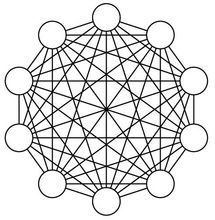
\includegraphics[scale=0.9]{{figures/hopfield_network.jpg}}
\caption{霍普菲尔德网络}
\label{fig:hopfield_network}
\end{figure}

\subsubsection{霍普菲尔德网络的定义}
一个霍普菲尔德网络由$N$个神经元构成,每个神经元的激发函数是符号函数,于是每个神经元有两个状态——激发态和静息态,两种状态在数学上的值分别定义为$1$和$-1$;接下来再定义神经元$j$到神经元$i$的连接权重为$\MW_{ij}$,则所有的参数$\MW_{ij}$构成了连接矩阵$\MW$。霍普菲尔德网络中的连接$\MW_{ij}$有两个约束条件:
\begin{itemize}
	\setlength{\itemsep}{0pt}
    \setlength{\parsep}{0pt}
    \setlength{\parskip}{0pt}
	\item 对称性: $\MW_{ij}$ = $\MW_{ji}$
	\item 不存在自连接: $\MW_{ii} = 0$
\end{itemize}
设神经元$i$的状态为$x_{i}$则
\begin{eqnarray}
x_{i} =
\begin{cases}
1   & \quad  \sum_{j}^{} \MW_{ij}x_{j} \geq 0\\
-1  & \quad  \sum_{j}^{} \MW_{ij}x_{j} < 0 
\end{cases} \nonumber
\end{eqnarray}
即
\begin{eqnarray}
x_{i} = \mathop{\rm sgn}(\sum_{j}^{} \MW_{ij}x_{j}) \nonumber
\end{eqnarray}

可以看出,假如给霍普菲尔德网络一个初始状态,网络将会不断的自我演化更新直至稳态或震荡。网络状态的更新有两种方式:
\begin{itemize}
	\setlength{\itemsep}{0pt}
    \setlength{\parsep}{0pt}
    \setlength{\parskip}{0pt}
    \item 同步更新:所有的神经元同时计算在当前时刻所接收到的输入,之后在同一时刻一齐更新到新的状态。
	\item 异步更新:按照依次或随机选择一个神经元,根据其接收的输入更新其状态。
\end{itemize}
当满足连接权重的对称性和不存在自连接两个约束条件时,使用异步更新的方式更新网络状态,可以保证霍普菲尔德网络收敛(霍普菲尔德网络并非本书讨论的重点内容,因此在本章节将不再深入的讨论其收敛性证明)。下面我们要引入\textbf{能量}的概念。

\subsubsection{回声网络与能量}
我们通过一种更加简单的模型——双向关联记忆网络(Bidirectional Associative Memory, BAM)来引入能量。BAM又称为回声网络(Resonance Network),如图\ref{fig:bam},其基本组成单元与霍普菲尔德网络的神经元一样,激发函数为符号函数。回声网络可以看作是一个两层网络,两层之间全连接,层内无连接,也不存在自连接。
\begin{figure}[ht]
\centering
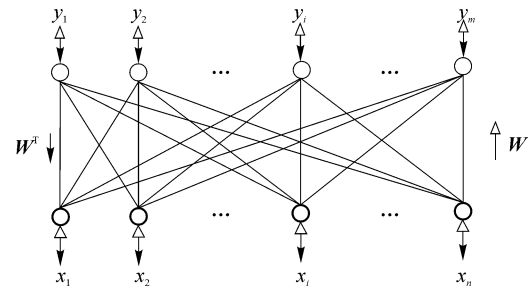
\includegraphics[scale=0.8]{{figures/bam.png}}
\caption{回声网络}
\label{fig:bam}
\end{figure}

图\ref{fig:bam}中所示的回声网络由两层构成,分别记为$x$层和$y$层。设其输入为$n$维行向量$\Vx$,输出为$k$维行向量$\Vy$,两层之间$n \times k$的权重矩阵为$\MW$,网络第一次更新时更新$y$层得到$\Vy_{(0)}$,则有
\begin{eqnarray}
y_{(0)} = \mathop{\rm sgn}(\Vx_{(0)}\MW) \nonumber
\end{eqnarray}
接着以$\Vy_{(0)}$作为输入,向左传更新$x$层,得到$\Vx_{(0)}$
\begin{eqnarray}
\Vx_{(1)}^\top = \mathop{\rm sgn}(\MW\Vy_{(0)}^\top)\nonumber
\end{eqnarray}
再以$\Vx_{(1)}$作为输入,向右传更新$y$层,得到$\Vy_{(1)}$
\begin{eqnarray}
\Vy_{(1)} = \mathop{\rm sgn}(\Vx_{1}\MW)\nonumber
\end{eqnarray}
归纳可得:
\begin{eqnarray}
\Vy_{(i)} &=& \mathop{\rm sgn}(\Vx_{(i)}\MW)\nonumber\\
\Vx_{(i)}^\top &=& \mathop{\rm sgn}(\MW\Vy_{(i)}^\top)\nonumber
\end{eqnarray}
如果BAM最终达到了稳定状态,即向量$\Vx$和$\Vy$都不再发生变化,记此时的$\Vx$,$\Vy$分别为$\Vx_{(m)} \Vy_{(m)}$,则有
\begin{eqnarray}
\Vy_{(m)} = \mathop{\rm sgn}(\Vx_{(m)}\MW) \quad \quad \Vx_{(m)}^\top = \mathop{\rm sgn}(\MW\Vy_{(m)}^\top)\nonumber
\end{eqnarray}
下面我们开始逐步引入能量。首先,定义一个关于$\Vx_{i}$的“激发向量”(excitation vector)$\Ve$,那么对于任意一对向量$(\Vx_{(i)},\Vy_{(i)})$有:
\begin{eqnarray}
\Ve^\top = \MW\Vy_{(i)}^\top\nonumber
\end{eqnarray}

如果$(\Vx,\Vy)$是最终的稳定向量对,则满足
\begin{eqnarray}
\mathop{\rm sgn}(\Ve) = \Vx\nonumber
\end{eqnarray}
直观上,如果向量$\Ve$想要满足这个条件,那么它每一项的符号都需要与$\Vx$相同,意味着$\Ve$足够靠近$\Vx$。可以想象一下,在二维空间,$\Ve$和$\Vx$落在同一个象限,在三维空间,$\Ve$和$\Vx$落在同一个卦限,以此类推,维数越高则对$\Ve$的约束越强。根据内积的定义,对于同样长度的$\Ve$,越靠近$\Vx_{0}$,两者的内积越大,因此是否可以使用$\Vx$和$\Ve$的内积来作为一个衡量回声网络收敛到稳态的指数呢?内积
\begin{eqnarray}
\langle\Vx,\Ve\rangle 
&=& \Vx\Ve^\top\nonumber\\
&=& \Vx\MW\Vy^\top\nonumber\\
&=& \Vx(\sum_{j=1}^{k}\MW_{1j}\Vy_{j},\sum_{j=1}^{k}\MW_{2j}\Vy_{j},\cdots,\sum_{j=1}^{k}\MW_{nj}\Vy_{j})\nonumber\\
&=& (\Vx_{1},\Vx_{2},...,\Vx_{n})(\sum_{j=1}^{k}\MW_{1j}\Vy_{j},\sum_{j=1}^{k}\MW_{2j}\Vy_{j},\cdots,\sum_{j=1}^{k}\MW_{nj}\Vy_{j})\nonumber\\
&=& \sum_{i=1}^{n}\Vx_{i}\sum_{j=1}^{k}\MW_{ij}\Vy_{j}\nonumber
\end{eqnarray}
$\Vx_{i}$和$\Vy_{j}$的取值只有$\pm1$,在回声网络处于稳态时,对于每一个$\Vx_{i}\sum_{j=1}^{k}\MW_{ij}\Vy_{j}$,$\Vx_{i}$与$\sum_{j=1}^{k}\MW_{ij}\Vy_{j}$的符号相同,则有每一个$\Vx_{i}\sum_{j=1}^{k}\MW_{ij}\Vy_{j}\geq0$,固定$\MW$和$\Vy_{0}$改变$\Vx_{0}$中某一项$\Vx_{s}$的符号(记为$\Vx_{s}^{'}$),则对应的$\Vx_{s}^{'}\sum_{j=1}^{k}\MW_{sj}\Vy_{j}\leq0$,于是有
\begin{eqnarray}
\sum_{i=1}^{n}\Vx_{i}\sum_{j=1}^{k}\MW_{ij}\Vy_{j} \geq \sum_{i=1,i\neq s}^{n}\Vx_{i}\sum_{j=1}^{k}\MW_{ij}\Vy_{j} + \Vx_{s}^{'}\sum_{j=1}^{k}\MW_{sj}\Vy_{j}\nonumber
\end{eqnarray}
由此可知,回声网络处于稳态时,$\Vx_{0}$和$\Ve$的内积最大。对于一般的物理系统,能量越低越稳定,因此使用内积的相反数作为能量的定义。于是对回声网络定义能量函数(Energy Function)。给定$\MW$,回声网络在某一时刻的$x$层输出$\Vx$和$y$层的输出$\Vy$,此时回声网络的能量函数定义为:
\begin{eqnarray}
E(\Vx,\Vy) = -\frac{1}{2}\Vx\MW\Vy^\top
\end{eqnarray}
所以对于一个回声网络,稳定态是它能量最小的状态($\frac{1}{2}$项与其他公式中的$\frac{1}{2}$一样是为了方便计算)。

现在我们把回声网络的能量函数推广到更一般的情况。若神经元的激发函数是一个阶跃函数,此时只需对能量函数进行一点点扩展即可。位于左边的$n$维向量$\Vx$和位于右边的$k$维向量$\Vy$分别各增加一维得到$(\Vx_{1},\cdots,\Vx_{n},1)$和 $(\Vy_{1},\cdots,\Vy_{n},1)$。连接权重矩阵$\MW$增加一行一列,与$\Vx$相关的阶跃函数阈值$\theta_{l}$对应写在$\MW$的第$k+1$列上,与$\Vy$相关的阶跃函数阈值${\theta_{r}}$对应写在$\MW$的第$n+1$行,$\MW$对角线上的元素依然保持为$0$。扩展后的能量函数为:
\begin{eqnarray}
E(\Vx,\Vy) = -\frac{1}{2}\Vx\MW\Vy^\top + \frac{1}{2}\theta_{r}\Vy^\top + \frac{1}{2}\Vx\theta_{l}^\top
\end{eqnarray}
下面直接根据回声网络的能量函数推出霍普菲尔德网络的能量函数。

\subsubsection{霍普菲尔德网络的能量函数}
霍普菲尔德网络与回声网络不同,它是一个全连接的网络,没有x层和y层之分。但我们可以利用霍普菲尔德网络的结构特点来把它看作是一个回声网络来处理:
\begin{enumerate}
	\setlength{\itemsep}{0pt}
    \setlength{\parsep}{0pt}
    \setlength{\parskip}{0pt}
	\item 霍普菲尔德网络只有一个$x$层。
	\item 在一个时刻内使用同步更新的方式更新网络。
	\item 假设在$t$时刻之内,$x$层中的所有神经元逐一完成了更新,那么它们($\Vx_{(t)}$)将在下一个时刻作为输入层传递给$t+1$时刻的自己($\Vx_{t+1}$);而它们($\Vx_{t}$)的输入可以看作来自$t-1$时刻的自己($\Vx_{t-1}$)。
	\item 把$\Vx_{t}$层看作回声网络中的$x$层,把$\Vx_{t+1}$层看作回声网络中的$y$层,那么在$t$到$t+1$时刻,完成了一次从$x$层到$y$层的传递更新。
	\item 更进一步,$t$为奇数时$x_{t}$作为x层,$t$为偶数时$x_{t}$作为y层,于是同步更新的Hopfield Network就转化成了一个回声网络。
\end{enumerate}
我们在本书第二章求解循环神经网络的时候已经用到过这种把网络在时间上展开的方法。现在可以直接使用回声网络的能量函数来描述霍普菲尔德网络。因为此时的$y$层就是$x$层自己,所以$\Vx$的阈值${\theta}={\theta_{l}}={\theta_{r}}$。那么霍普菲尔德网络的能量函数为:
\begin{eqnarray}
E(\Vx) 
&=& -\frac{1}{2}\Vx\MW{x}^\top + \frac{1}{2}{\theta}\Vx^\top + \frac{1}{2}\Vx{\theta}^\top\nonumber\\
&=& -\frac{1}{2}\Vx\MW{x}^\top + {\theta}\Vx^\top
\end{eqnarray}
把上式中的矩阵和向量展开,霍普菲尔德网络的能量函数还可以表示成:
\begin{eqnarray}
E(\Vx) = -\frac{1}{2}\sum_{j=1}^{n}\sum_{i=1}^{n}\MW_{ij}\Vx_{i}\Vx_{j} + \sum_{i=1}^{n}\theta_{i}\Vx_{i}
\end{eqnarray}
可以看出霍普菲尔德网络的能量函数是一个二次型,所以往往会有局部最优解。如何避免网络在收敛的过程中陷入局部最优呢?一个很直观的想法是引入概率,从而给网络一定的机会跳出局部最优。把概率引入霍普菲尔德网络并增加一些新的“组件”之后,我们将得到玻尔兹曼机。

\subsection{玻尔兹曼机}
\subsubsection{概率}
我们已经看到,当到霍普菲尔德网络达一个局部最优之后,网络的状态更新便停止了。如果这个局部最优不是全局最优(很可能不是),那么网络永远不能收敛到全局最优。自然而然地我们想到使用概率来给网络一个继续“探寻”下去的机会。如果每个单元(在玻尔兹曼机中通常把神经元称为单元)在确定自己的状态时并非完全取决于它所接收到的输入,而是根据接收的输入以一定的概率来随机产生某个状态,便可以达到这个目的。那么如何去做呢?下面我们要借助一套物理学上的工具来实现我们的目标。

物理学中有一个描述气体分子系统的工具叫玻尔兹曼分布(Boltzmann Distribution)。玻尔兹曼分布首次把统计学引入了物理学中,使用概率把宏观的系统能量和微观的分子状态联系在了一起,并找到了概率和能量的关系。在霍普菲尔德网络中我们已经有了能量,再利用玻尔兹曼分布中能量和概率的关系,便可以把概率引入神经网络。

假设网络中某单个单元$x_{k}$可能的状态有$0$(静息态)和$1$(激发态)两种(注意此时静息态的值为$0$,不是$-1$,这只是为了计算方便,就像在逻辑回归中我们常用$1$和$0$来标记正负样本,而在支持向量机中常用$1$和$-1$来标记正负样本),当$x_{k}$的状态从0($x_{k}=0$)变到1($x_{k}'=1$)时,整个网络能量的变化量为$\Delta E_{i}$。根据上一节我们推出的霍普菲尔德网络能量函数可知
\begin{eqnarray}
\Delta E_{k} 
&=& E(\Vx) - E(\Vx') \nonumber\\
&=& -(\Vx_{k} - \Vx_{k}')(\sum_{i=1}^{n}\MW_{ki} - \theta_{k}) \nonumber\\
&=& \sum_{i=1}^{n}\MW_{ki} - \theta_{k}
\end{eqnarray}
根据玻尔兹曼分布的性质——系统某个状态的能量与该状态出现概率的自然对数的相反数成正比,即$E=-T\log(p)$,有
\begin{eqnarray}
\Delta E_{k} 
&=& E_{\Vx_{k}=0} - E_{\Vx_{k}=1} \nonumber\\
&=& -T\log (p_{\Vx_{k}=0}) - (-T\log (p_{\Vx_{k}=1}))\nonumber
\end{eqnarray}
因为$p_{\Vx_{k}=0}+p_{\Vx_{k}=1}$则
\begin{eqnarray}
\Delta E_{k} = -T\log (1-p_{\Vx_{k}=1}) - (-T\log (p_{\Vx_{k}=1}))\nonumber \\
\frac{\Delta E_{k}}{T} = \log (p_{\Vx_{k}=1}) - \log (1-p_{\Vx_{k}=1})\nonumber \\
\frac{\Delta E_{k}}{T} = \log (\frac{p_{\Vx_{k}=1}}{1-p_{\Vx_{k}=1}})\nonumber \\
-\frac{\Delta E_{k}}{T} = \log (\frac{1-p_{\Vx_{k}=1}}{p_{\Vx_{k}=1}})\nonumber \\
-\frac{\Delta E_{k}}{T} = \log (\frac{1}{p_{\Vx_{k}=1}}-1)\nonumber \\
\exp(-\frac{\Delta E_{k}}{T}) = \frac{1}{p_{\Vx_{k}=1}}-1\nonumber \\
\end{eqnarray}
最终得到神经元$x_{k}$处于激发态($x_{k}=1$)的概率
\begin{eqnarray}
p_{\Vx_{k}=1} = \frac{1}{1+\exp (-\frac{\Delta E_{k}}{T})}
\end{eqnarray}
上式中的比例系数$T$可以看作是网络的“温度”。需要特别注意的是,只有当网络收敛到稳定状态时单元所处的状态才会服从玻尔兹曼分布,对应于物理系统的热平衡(Thermal Equilibrium)。

\subsubsection{概率的意义和隐藏单元}
到目前为止,引入概率之后的网络(姑且称为“随机化的霍普菲尔德网络”)已经有能力跳出局部最优。只要时间足够长,网络将会遍历所有可能的状态。如果把单元看作气体分子,那么整个网络则是一个服从玻尔兹曼分布的系统。而服从某种分布的网络可以用来模拟现实世界的某种服从概率分布/统计的行为。什么意思呢?想象一下,我们对现实世界中的某一个事物进行观察,并使用一组变量来表示观察结果。最终收集到的一系列结果会服从某种分布。然后我们希望使用神经网络来模拟我们的观测结果。这就相当于使用神经网络构建一个网络内部的模型,该模型所服从的分布与观察结果所服从的分布接近甚至相同。如果能够建立这样一个网络,将会非常有用。例如可以通过网络来得到更多的结果而不必进行更多的观测;或者对网络本身进行研究,从而得到对现实世界中该事物产生这样一组观测结果的过程更加深入的认识。

但是,“随机化的霍普菲尔德网络”对于绝大多数的情况完全不能够胜任。这是因为网络本身的结构——“随机化的H霍普菲尔德网络”的单元数目与“描述观测结果的变量”数目相等——造成的。根据玻尔兹曼分布,网络处于热平衡态时,某种状态的出现概率只取决于于它的能量:
\begin{eqnarray}
P_{\alpha} = \frac{\exp(-E_{\alpha})}{\sum_{\beta}\exp(-E_{\beta})}\nonumber
\end{eqnarray}
其中$P_{\alpha}$是处于平衡态时网络状态为$\alpha$的概率,分母是所有可能的状态求和(分母除以比例系数$T$之后是概率,再求和其实就是1)。网络的行为特性由它的连接权重$\MW_{ij}$决定。连接权重$w_{ij}$的变化对网络进入某种状态的概率的影响可以通过该状态的概率对连接权重求偏导得到:
\begin{eqnarray}
\frac{\partial\log P_{\alpha}}{\partial \MW_{ij}} = \frac{1}{T}(\Vx_{i}^{\alpha}\Vx_{j}^{\alpha}-\sum_{\beta}P_{\beta}\Vx_{i}^{\beta}\Vx_{j}^{\beta}) \nonumber
\end{eqnarray}
其中$\Vx_{k}^{\gamma}$表示第$k$个单元$\Vx_{k}$在网络处于状态$\gamma$时的状态(推导过程可以参见玻尔兹曼机的求解过程)。由该式可见,连接权重只通过单元对$(\Vx_{i}\Vx_{j})$影响网络进入某种状态的概率。这意味着“随机化的霍普菲尔德网络”只能捕捉到现实世界中二阶及以下的结构,对更高阶的结构无能为力。例如在一个三单元网络看来,一组状态$((0,0,0),(0,1,1),(1,0,1),(1,1,0))$与另一组状态$((1,1,1),(1,0,0),(0,1,0),(0,0,1))$是一样的,因为他们的均值与内部相关性是相等的。如何解决这个问题?一个直观的想法就是引入更多的单元去捕捉那些高阶的结构。这些后来引入的单元并不用来表示现实世界的某个观测变量,它们被称为隐藏单元(Hidden Units);而原本的那些对应于观测结果的单元被称为可见单元(Visible Units)。这种“加入隐藏单元的随机化霍普菲尔德网络”就是玻尔兹曼机(图\ref{fig:bm})。
\begin{figure}[ht]
\centering
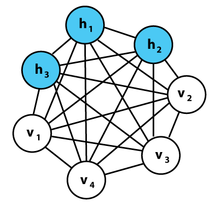
\includegraphics[scale=0.8]{{figures/bm.png}}
\caption{玻尔兹曼机}
\label{fig:bm}
\end{figure}

玻尔兹曼机中的可见单元可以看作是网络中与现实世界的接口,而现实世界中得到的观测结果变量同样可以看作是现实世界中与网络的接口。网络内部的模型建立的越好,两个接口越接近。所谓的“两个接口接近”事实上指的是:现实世界中的观测结果变量所服从的真实分布,与网络中的可见单元所服从的分布相似。我们再一次遇到了衡量两个分布相似度的问题。在玻尔兹曼机中,我们使用KL距离,这其实意味着玻尔兹曼机是在\textbf{通过最大似然估计直接学习样本数据真实分布}。

把可见单元记为$\Vv$,隐藏单元记作$\Vh$,则$|\Vv|$个可见单元可能的状态共有$2^{|\Vv|}$个,相应地,观测结果变量可能的状态也有$2^{|\Vv|}$个。
% 把观测结果变量进入第$\alpha$个状态的概率记为$P_{r}(\Vv_{\alpha})$,可见单元进入同一个状态的概率记为$P_{\Vw}(\Vv_{\alpha})$。
观测结果的$P_{r}(\Vv)$是目标分布,我们希望网络的$P_{\Vw}(\Vv)$尽可能地靠近前者。二者的KL距离为
\begin{eqnarray}
D_{KL}(P_{r}(\Vv)\|P_{\Vw}(\Vv)) = \sum_{\Vv}P_{r}(\Vv)\log\frac{P_{r}(\Vv)}{P_{\Vw}(\Vv)}
\end{eqnarray}
观测结果的分布$P_{r}(\Vv)$是已知的。可见单元的分布$P_{\Vw}(\Vv)$由该状态对应的能量$E_{\Vv,\Vh}$决定,而$E_{\Vv,\Vh}$唯一由网络的连接权重$\Vw_{ij}$确定。所以二者的KL距离是关于连接权重$\Vw_{ij}$的函数,于是便可以采用梯度下降法来训练网络。由于篇幅所限,本书就不再继续推导下去了,感兴趣的读者可以阅读相应的文献,在这里我们直接给出结果:
\begin{eqnarray}
\frac{\partial D_{KL}}{\partial \Vw_{ij}} = -\frac{1}{T}(p_{ij} - p'_{ij})
\end{eqnarray}
其中$p_{ij}$是网络到达平衡态后固定可见单元时$(x_{i},x_{j})$同时被激发的概率;$p'_{ij}$是网络到达平衡态时$(x_{i},x_{j})$同时被激发的概率;单元$x_{i}$为某一个可见单元或隐藏单元。

可以看出在训练玻尔兹曼机时,每次调整完连接权重$\Vw_{ij}$都要等待网络进入平衡态后,分别统计$p_{ij}$和$p'_{ij}$,才能进行一次梯度下降更新,训练效率极其低下。当网络的规模变大、结构越发复杂的时候,网络进入平衡态需要很长时间,所以玻尔兹曼机在实际使用中的效果并不理想。若想使得玻尔兹曼机能够用于实践,就不得不对其网络复杂度进行控制。网络复杂度是由单元和单元间的连接决定的,在保持单元数目不变的前提下,那就只能对单元间连接的数目进行限制了——受限玻尔兹曼机。

\subsection{受限玻尔兹曼机}
去掉玻尔兹曼机中可见单元之间的连接,再去掉隐藏单元之间的连接,就得到了受限玻尔兹曼机。受限玻尔兹曼机是一个双层无向网络,结构与我们在回声网络很相似(图\ref{fig:rbm})。通常受限玻尔兹曼机中单元的激发函数是sigmoid函。
\begin{figure}[ht]
\centering
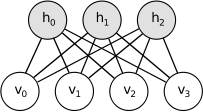
\includegraphics[scale=0.9]{{figures/rbm.png}}
\caption{受限玻尔兹曼机}
\label{fig:rbm}
\end{figure}

受限玻尔兹曼机中能量的定义与玻尔兹曼机保持一致。设网络由$m$个可见单元和$n$个隐藏单元构成,则受限玻尔兹曼机的能量定义为
\begin{eqnarray}
E(\Vv,\Vh) = -\sum_{i=1}^{n}\sum_{j=1}^{m}\Vw_{ij}\Vh_{i}\Vv_{j} - \sum_{j=1}^{m}\Vb_{j}\Vv_{j} - \sum_{i=1}^{n}\Vc_{i}\Vh_{i}
\end{eqnarray}
其中$\Vw_{ij}$是可见单元$\Vv_{j}$与隐藏单元$\Vh_{i}$之间的连接权重,$\Vb_{j}$和$\Vc_{i}$分别是可见单元$\Vv_{j}$与隐藏单元$\Vh_{i}$的偏置。注意,当该项定义为“阈值”的时候,它大于$0$,而当该项定义为“偏置”的时候,它小于$0$。因此受限玻尔兹曼机中能量函数的“偏置项”与玻尔兹曼机中的“阈值项”的符号不同,但意义是一样的。

受限玻尔兹曼机的求解比玻尔兹曼机高效很多,常用的有Gibbs采样、变分法、对比分歧算法(Constrastive Divergence)等等。受限玻尔兹曼机这样一个“浅网络”表达能力不够强,随着深度学习的崛起,受限玻尔兹曼机已经用的比较少了。